\chapter{Tworzenie aplikacji zbierającej dane pomiarowe}

Aplikacja do odbierania danych z czujnika, ich obrabiania oraz przesłania do żądanej bazy danych została całkowicie napisana w języku C. Jest to jeden z języków najczęściej używanych do obsługi systemów wbudowanych. Posiada ogromną ilość bibliotek, które usprawniają pisanie kodu i aplikacji. Dzięki stworzonym bibliotekom można skupić się na tworzeniu programu zamiast tracić czas na tworzenie każdej najmniejszej funkcjonalności od początku.

Główny program stacji pogodowej zawiera w sobie podprocedury do obsługi czujników oraz transmitowaniu zebranych danych bo bazy. Odpowiedni podział na podfunkcję sprawia, że kod jest czytelniejszy oraz łatwiej jest go zrozumieć dla osób postronnych. Taka zasada została uwzględniona przy tworzeniu aplikacji do obsługi pomiarów meteorologicznych.

Kwestie bezpieczeństwa również zostały zaimplementowane. W kodzie istnieje kilkanaście różnych wartości oznaczających błędy, jeżeli którykolwiek z nich będzie miał miejsce, nie pozwoli to na dalsze wykonywanie programu. Aplikacja w takim przypadku zostanie zatrzymana, a problem, który nastąpił zostanie zgłoszony obsługującemu w celu jego wyeliminowania.

Kody błędów są zwracane w przypadku, gdy jakaś część programu zostanie wykonana niepoprawnie. Może to być spowodowane chwilowym brakiem łączności z czujnikami lub brakiem dostępu do internetu, aby dodać pomiary do bazy danych. Mogą również wystąpić błędy systemowe, jak np. niepozwolenie na otwarcie pliku. Każdy z problemów może okazać się groźny dla wykonywanej aplikacji, dlatego musi nastąpić zamknięcie całej funkcjonalności.

Na rysynku \ref{fig:diagram_program} przedstawiony został schemat blokowy głównej funkcji programu stacji pogodowej. Widać na nim, że w przypadku błędu, wszystko zostanie poprawnie zakończone, aby nie spowodować uszkodzenia jakiejkolwiek części układu pomiarowego.

\begin{figure}[h]
\centering
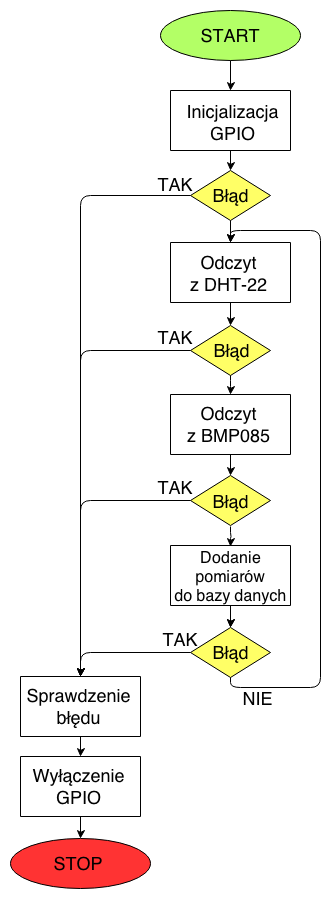
\includegraphics[scale=0.6]{diagram_program}
\caption{Diagram programu głównego stacji pogodowej}
\label{fig:diagram_program}
\end{figure}

\section*{Używanie MySQL z poziomu języka C}
Baza danych MySQL zostanie szerzej przedstawiona w następnym rozdziale.

Posiadając odebrane prawidłowe pomiary z czujników, należy je następnie zamieścić w bazie danych, aby były one dostępne do wyświetlania lub analizowania. W tym celu potrzebny jest sposób na umieszczenie danych do tej bazy z poziomu programu napisanego w języku C.

Producent bazy danych MySQL udostępnił interfejs komunikacyjny bazy, gotowy do zaimplementowania w C. Nazywa się on MySQL C API i jest dostępny dla wszyskich użytkowników za darmo. MySQL C API jest to biblioteka funkcji, która umożliwia komunikację programu z bazą danych MySQL.

W celu skorzystania z udostępnionej biblioteki najpierw należy ją skompilować do użytku na mikrokomputerze BeagleBone Black. Na stronie głównej projektu MySQL są do ściągnięcia źródła tej biblioteki, po ich pobraniu należy przy pomocy cross-kompilatora skompilować je do biblioteki.

Dodatkowo należy również zainstalować obsługę MySQL na mikrokomputerze, cała procedura instalacji jest ujęta w jednej komendzie, w konsoli należy wpisać:\newline
\emph{sudo apt-get install libmysqlclient-dev}

Po poprawnym zainstalowaniu i skompilowaniu biblioteki można przejść do kompilacji całego projektu, który będzie łączył się z podaną bazą danych oraz wyciągał z niej i wpisywał do niej rekordy.

Korzystanie z API przygotowanego przez producenta bazy danych jest bardzo proste i wymaga niewielkiej wiedzy początkowej. Dokumentacja jest opisana bardzo jasno oraz można znaleźć dużo poradników na temat używania interfejsu komunikacji z bazą danych.

Diagram przedstawiony na następnej stronie na rysunku \ref{fig:diagram_mysql} ukazuje schemat blokowy funkcji łączącej się z bazą danych, wstawianiu danych uzyskanych w nowym pomiarze oraz pobraniu z bazy okresu próbkowania między pomiarami.

Zgodnie z zasadą pisania całego oprogramowania, każdy napotkany błąd jest przekazywany dalej, a w głównej funkcji obsługi stacji pogodowej jest on wyświetlany oraz kończony jest program. Gdy problem nastąpi po nawiązaniu połączenia z bazą, połączenie to musi zostać zakończone, aby nie doszło do wycieków pamięci.

\begin{figure}[h]
\centering
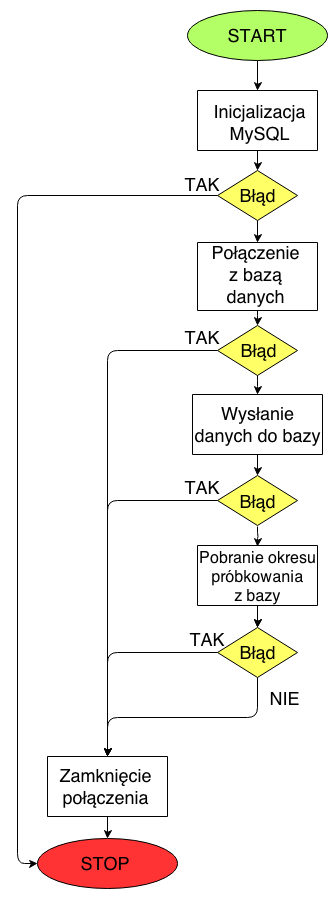
\includegraphics[scale=0.6]{diagram_mysql}
\caption{Diagram programu dodającego dane do bazy MySQL}
\label{fig:diagram_mysql}
\end{figure}
